\documentclass[12pt,letterpaper,boxed]{hmcpset}
\usepackage{float}
\restylefloat{figure}
\usepackage{graphicx}
\usepackage{amsmath}


\name{Lujia Zhang}
\class{CSSE 477}
\mailbox{CM 1405}
\assignment{Assignment 8}

\begin{document}

\section*{Snapshots}
\begin{figure}[H]
  \centering
  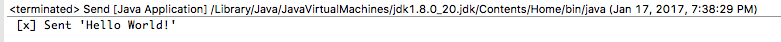
\includegraphics[width = 1.0\textwidth]{1.png}
\end{figure}
\begin{figure}[H]
  \centering
  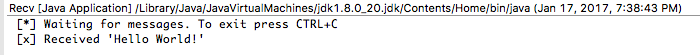
\includegraphics[width = 1.0\textwidth]{2.png}
\end{figure}
\begin{figure}[H]
  \centering
  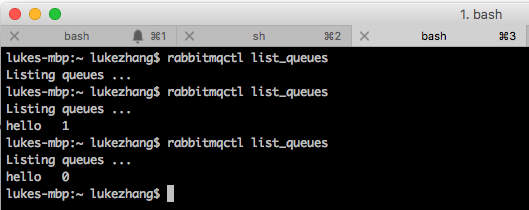
\includegraphics[width = 1.0\textwidth]{3.png}
\end{figure}
\begin{figure}[H]
  \centering
  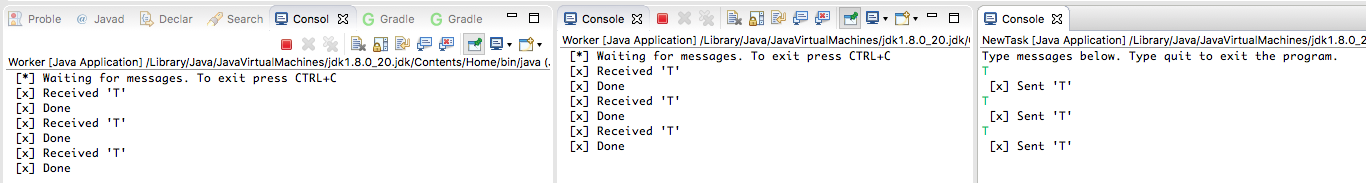
\includegraphics[width = 1.0\textwidth]{4.png}
\end{figure}
\begin{figure}[H]
  \centering
  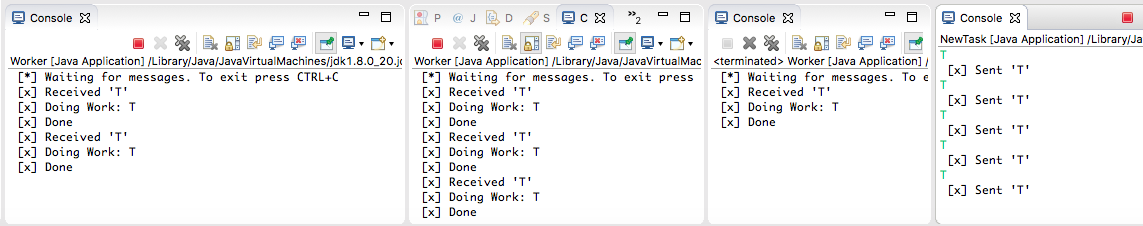
\includegraphics[width = 1.0\textwidth]{5.png}
\end{figure}
\begin{figure}[H]
  \centering
  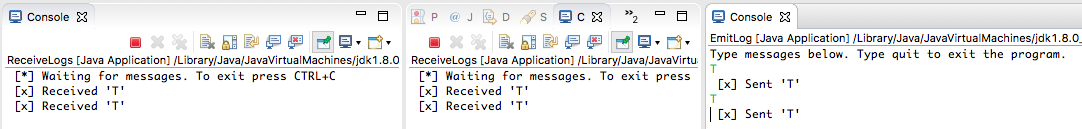
\includegraphics[width = 1.0\textwidth]{6.png}
\end{figure}
\begin{figure}[H]
  \centering
  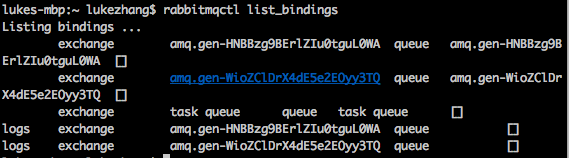
\includegraphics[width = 1.0\textwidth]{7.png}
\end{figure}
\begin{figure}[H]
  \centering
  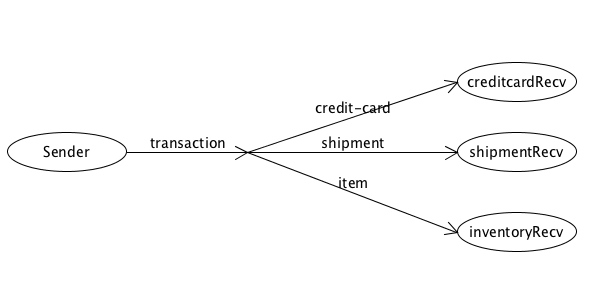
\includegraphics[width = 1.0\textwidth]{9.png}
\end{figure}
\begin{figure}[H]
  \centering
  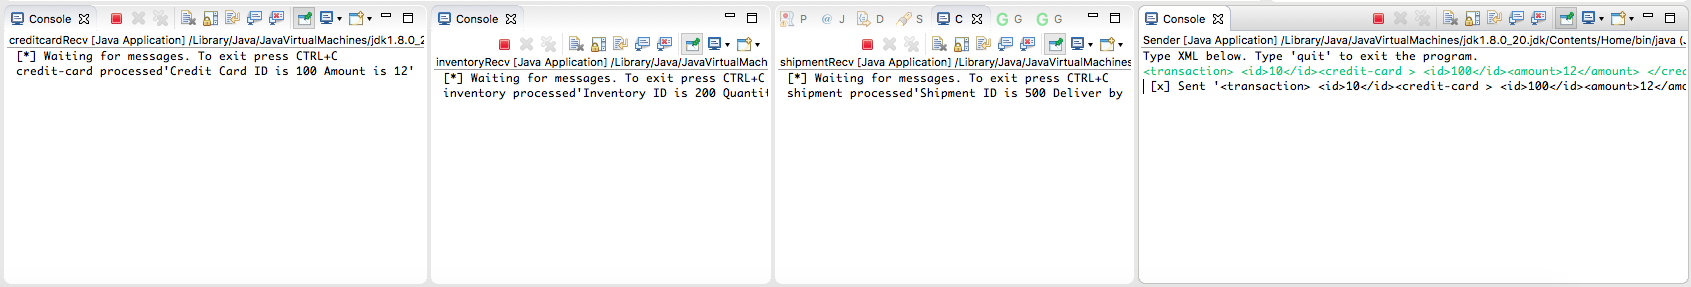
\includegraphics[width = 1.0\textwidth]{8.png}
\end{figure}
\end{document}